\documentclass[11pt,letterpaper]{article}

\usepackage[margin=0.6in]{geometry}
\usepackage{enumitem}
\usepackage{amsmath}
\usepackage{xcolor}
\usepackage{tikz}
\usetikzlibrary{decorations.pathmorphing, decorations.pathreplacing, calc, arrows.meta}

\pagestyle{empty}
\setlength{\parindent}{0pt}

% Answer block, set in a contrasting color
\newenvironment{answer}{\par\vspace{4pt}\color{blue!60!black}\textbf{Answer:}\ }{\par\vspace{4pt}}

\begin{document}

\begin{center}
    {\Large \textbf{16.07 Dynamics --- Quiz 6: Spacecraft Dynamics and Thruster Allocation (Solutions)}}\\[4pt]
\end{center}

\vspace{10pt}
\begin{enumerate}[label=\textbf{\arabic*.}, leftmargin=*, itemsep=4pt]

\item A single thruster is mounted on a rigid spacecraft at position ${}^{B}\mathbf{r}$ relative to the center of mass $O$. It pushes the spacecraft along the unit vector ${}^{B}\mathbf{d}$ with thrust $u \ge 0$, as shown below. Write the $6\times1$ input Jacobian $\mathbf{B}$ that maps $u$ into the wrench $\bigl[\,{}^{B}\mathbf{F}^T\;\; {}^{B}\boldsymbol{\tau}^T\bigr]^T = \mathbf{B}\,u$, in terms of ${}^{B}\mathbf{r}$ and ${}^{B}\mathbf{d}$.

\vspace{6pt}
\begin{minipage}[c]{0.42\linewidth}
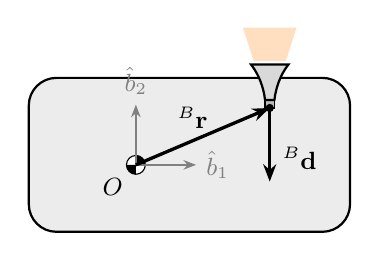
\begin{tikzpicture}[scale=0.85]
    % Spacecraft body
    \filldraw[fill=gray!15, draw=black, thick, rounded corners=10pt] (-1.6,-1.0) rectangle (3.2,1.3);
    % Center of mass
    \filldraw[fill=white] (0,0) circle (4pt);
    \fill (0,0) -- ++(4pt,0) arc (0:90:4pt) -- cycle;
    \fill (0,0) -- ++(-4pt,0) arc (180:270:4pt) -- cycle;
    \node[below left, font=\small] at (-0.05,-0.05) {$O$};
    % Body axes
    \draw[-{Stealth[length=1.6mm]}, thick, gray] (0,0) -- (0.9,0) node[right, font=\small] {$\hat b_1$};
    \draw[-{Stealth[length=1.6mm]}, thick, gray] (0,0) -- (0,0.9) node[above, font=\small] {$\hat b_2$};
    % Thruster location
    \coordinate (P) at (2.0,0.85);
    \draw[-{Stealth[length=2.2mm]}, very thick] (0,0) -- (P);
    \node[font=\small] at (0.85,0.7) {${}^{B}\mathbf{r}$};
    % Thruster bell (exhaust points up, so the force on the spacecraft points down)
    \begin{scope}[shift={(P)}, rotate=90]
        \filldraw[fill=gray!55, draw=black] (0,-0.07) rectangle (0.12,0.07);
        \filldraw[fill=gray!30, draw=black, thick]
            (0.12,0.07) .. controls (0.3,0.09) and (0.5,0.16) .. (0.65,0.28)
            -- (0.65,-0.28) .. controls (0.5,-0.16) and (0.3,-0.09) .. (0.12,-0.07) -- cycle;
        \fill[orange!25] (0.7,0.24) -- (1.2,0.4) -- (1.2,-0.4) -- (0.7,-0.24) -- cycle;
    \end{scope}
    \filldraw (P) circle (1.5pt);
    % Force direction
    \draw[-{Stealth[length=2.2mm]}, very thick] (P) -- ++(0,-1.1);
    \node[font=\small, right] at ($(P)+(0.05,-0.75)$) {${}^{B}\mathbf{d}$};
\end{tikzpicture}
\end{minipage}\hfill
\begin{minipage}[c]{0.55\linewidth}
\color{blue!60!black}
\textbf{Answer:} \ $\mathbf{B} = \begin{bmatrix} {}^{B}\mathbf{d} \\ {}^{B}\mathbf{r}\times{}^{B}\mathbf{d} \end{bmatrix}$.

\vspace{4pt}
The force is ${}^{B}\mathbf{F} = u\,{}^{B}\mathbf{d}$, and it acts at ${}^{B}\mathbf{r}$, so the torque about $O$ is ${}^{B}\boldsymbol{\tau} = {}^{B}\mathbf{r}\times{}^{B}\mathbf{F} = u\left({}^{B}\mathbf{r}\times{}^{B}\mathbf{d}\right)$.
\end{minipage}
\vspace{6pt}

\item We wrote the translation dynamics of the Dragon in the inertial (ECI) frame. What if we instead wrote them in the body frame like we had previously in class for the quadrotor, with configuration $\mathbf{q} = \bigl[\,{}^{N}\mathbf{r}^T\;\; \mathbf{a}^T\bigr]^T$ and velocity $\mathbf{v} = \bigl[\,{}^{B}\dot{\mathbf{r}}^T\;\; {}^{B}\boldsymbol{\omega}^T\bigr]^T$? Which terms in the manipulator equation and kinematics would change? Circle them below and write a short explanation.
\begin{center}
\Large
$\dot{\mathbf{q}} \;=\; \mathbf{N}(\mathbf{q})\;\mathbf{v},
\qquad\qquad
\mathbf{M}(\mathbf{q})\;\dot{\mathbf{v}} \;+\; \mathbf{c}(\mathbf{q},\mathbf{v}) \;+\; \mathbf{g}(\mathbf{q}) \;=\; \mathbf{B}(\mathbf{q})\;\mathbf{u}.$
\end{center}

\begin{answer}
\textbf{$\mathbf{N}(\mathbf{q})$, $\mathbf{c}(\mathbf{q},\mathbf{v})$, $\mathbf{g}(\mathbf{q})$, and $\mathbf{B}(\mathbf{q})$ change. $\mathbf{M}$ does not.}

Here ${}^{B}\dot{\mathbf{r}} = \mathbf{A}(\mathbf{a})^T\,{}^{N}\dot{\mathbf{r}}$ is the velocity of the center of mass in body-frame components.
\begin{itemize}[leftmargin=1.5em, itemsep=1pt]
    \item $\mathbf{N}(\mathbf{q})$: the position $\mathbf{r}$ is still in $N$, so the velocity has to be rotated back, ${}^{N}\dot{\mathbf{r}} = \mathbf{A}(\mathbf{a})\,{}^{B}\dot{\mathbf{r}}$. The top-left block of $\mathbf{N}$ changes from $\mathbf{I}$ to $\mathbf{A}(\mathbf{a})$.
    \item $\mathbf{c}(\mathbf{q},\mathbf{v})$: the body frame rotates, so differentiating the velocity in $B$ adds the term $m\,{}^{B}\boldsymbol{\omega}\times{}^{B}\dot{\mathbf{r}}$ to the translational rows, which were zero before.
    \item $\mathbf{g}(\mathbf{q})$: gravity points toward the Earth's center, which is fixed in $N$, so in body components it has to be rotated by $\mathbf{A}(\mathbf{a})^T$. It now depends on the attitude as well as the position.
    \item $\mathbf{B}(\mathbf{q})$: the thrust force no longer has to be rotated into $N$, so $\mathbf{B}(\mathbf{q})$ becomes the constant body-frame input Jacobian $\mathbf{B}$.
    \item $\mathbf{M} = \operatorname{diag}(m\,\mathbf{I},\ \mathbf{J})$ is unchanged, and the rotational rows are unchanged, since Euler's equation was already written in $B$.
\end{itemize}
\end{answer}

\item To allocate thrust, we used the naive pseudoinverse solution $\mathbf{u} = \mathbf{B}^{+}\,{}^{B}\mathbf{w}_{\text{des}}$, and solved the quadratic program
\[
\underset{\mathbf{u}}{\text{minimize}} \;\; \tfrac12\,\mathbf{u}^T\mathbf{u}
\qquad \text{subject to} \qquad
\mathbf{B}\,\mathbf{u} = {}^{B}\mathbf{w}_{\text{des}}, \qquad
0 \le u_i \le u_{\max}.
\]
Recall that the pseudoinverse $\mathbf{B}^{+}\,{}^{B}\mathbf{w}_{\text{des}}$ gives the smallest $\lVert\mathbf{u}\rVert$ that satisfies $\mathbf{B}\,\mathbf{u} = {}^{B}\mathbf{w}_{\text{des}}$. Under what condition will the pseudoinverse solution be the same as the QP solution?

\begin{answer}
\textbf{When every entry of the pseudoinverse solution already satisfies the thrust limits, $0 \le u_i \le u_{\max}$.}

The pseudoinverse minimizes the same objective without the bounds on $u$, so if its solution already satisfies them, it is also the (unique) QP solution.
\end{answer}

\end{enumerate}

\end{document}
